\chapter{Исследование прототипа детектора для установки <<Лазерный поляриметр>>}
\label{sec:pol_examine}
\section{Конструкция детектора}
Для регистрации одиночных гамма--квантов, полученных обратным комптоновским рассеянием на пучках электронов, был спроектирован и изготовлен прототип детектора, использующего ГЭУ для усиления сигнала первичной ионизации. В конструкции применен тройной электрод с питанием от резистивного делителя. Основа детектора представляет собой многослойную плату из СТЭФ с массивом плоских металлических электродов, расположенных в её центральной части, которую можно видеть на Рис. \ref{fig:Pol_det_photo} 
\par Электроды поделены на группы, каждая из которых регистрируется отдельной считывающей платой. Всего считывающих плат десять, и они установлены в специальные многоканальные разъемы на периферии основной платы. Front-end электроника включает в себя быстрые АЦП и ПЛИС для работы с ними. Далее сигнал по USB подается на компьютер. На данный момент разрабатывается программное обеспечивающее взаимодействие всех 10 плат и одновременное считывание события с детектора. Решено было использовать для последующих экспериментов только одну из плат, т.к. вычитывание данных с неё уже отлажено. 
\par Электроды ГЭУ укреплены на рамках из 1.5 мм СТЭФ над считывающей структурой. Сверху на плату закрепляется герметичный кожух из СТЭФ с трубками для ввода и вывода газовой смеси. Сборка детектора осуществляется в корпусе из листового алюминия.
\par Данный детектор отличается от аналогов большей гранулярностью, что даст большую точность определения координат событий. (может ещё что написать)
\section{Особенности сбора и обработки сырых данных}
\label{sec:DAQ_raw_data}
Каналы детектора объединены в группы по 100 (центральная часть) или 120 (периферия) каналов. Каждая группа скоммутирована на отдельный разъем, к которому подключены два многоканальных АЦП. Одновременно можно вычитывать данные со всех каналов. При поступлении сигнала с триггера, схема начинает последовательно раз в 125 нс вычитывать заряд со всех каналов. Таким образом вычитывание происходит 100 раз. Каждый отсчет времени будем в дальнейшем называть <<кадром>>, а массив данных о заряде для каждого из каналов группы и каждого кадра из 100 назовем <<событием>>. 
\par Из-за технических особенностей схемы нулевой уровень сигнала составляет 7400 каналов АЦП. Сигнал, соответствующий пришедшей на электрод ионизации, представляет собой импульс отрицательной полярности, который имеет резкий передний фронт (1 кадр) и экспоненциально затухающий задний фронт (3-10 кадров в зависимости от суммарного заряда). Для последующей обработки сигнала, из него необходимо вычесть пьедестал. С этой целью в программе управления считывающей платой реализована возможность получения усредненных данных о пьедесталах, которые затем записываются в отдельный файл формата TXT. На Рис. \ref{pedestal_map} представлены гистограммы для пьедесталов одной считывающей платы.
\begin{figure}[H]
\begin{center}
	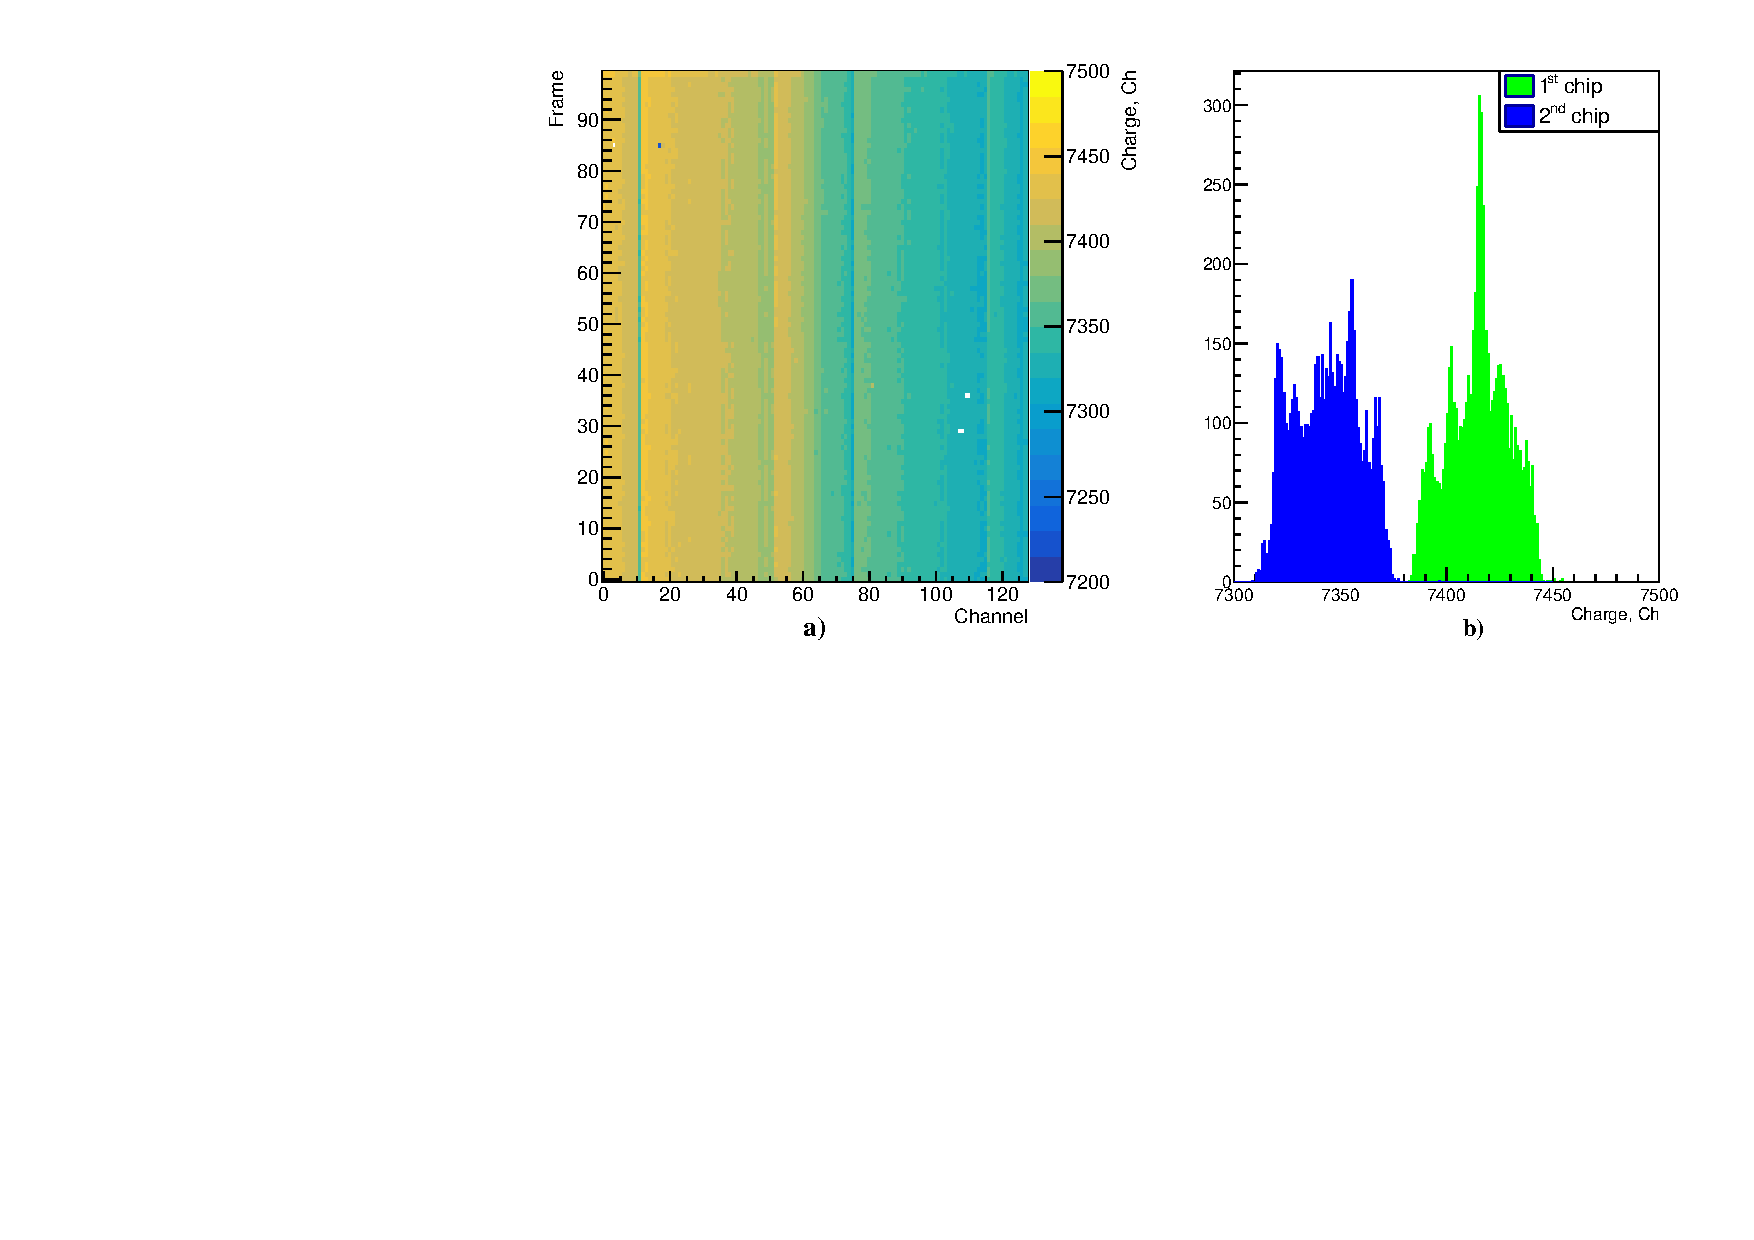
\includegraphics[width = 12cm]{img/pedestal_map.pdf}
	\caption{a): Карта пьедесталов АЦП. По горизонтальной оси обозначены номера каналов одной группы (Channel). По вертикальной оси --- кадры (Frame). Значения заряда показаны на цветовой шкале и лежат в пределах 7200--7500 каналов АЦП (Ch). b): Распределение заряда по каналам для первого и второго чипа считывающей платы}
	\label{pedestal_map}
\end{center}
\end{figure}
Можно заметить, что существует как разброс значений пьедестала в одном чипе, так и между чипами в плате. Поэтому решено было вычитать из сигнала пьедестал, соответствующий данному каналу.
\par События последовательно записываются в TXT--файл. Формат вывода следующий: строка соответствует одному кадру и состоит из 128 чисел. Всего таких строк в событии 100. 101--я строка содержит номер кадра, с которого началось вычитывание значений АЦП. Данная информация важна по следующей причине: микросхемы АЦП непрерывно вычитывают заряд с каналов, но ПЛИС возвращает событие только при активации триггера. Это сделано для того, чтобы исключить накопление заряда на входах АЦП и искажения данных о сигнале. Ввиду возможного разброса параметров электронных компонентов внутреннего pipeline АЦП, необходимо определять пьедесталы не только для каждого канала, но и для каждого кадра в канале. Поэтому номер канала в последней строке события дает необходимую привязку к физическим кадрам АЦП и позволяет правильно вычитать пьедесталы.
\par В ходе работы с прототипом детектора было обнаружено, что некоторые каналы имеют на порядок больший уровень шума, поэтому решено было их значения занулять и в анализе не использовать. 
\begin{figure}[H]
	\begin{center}
		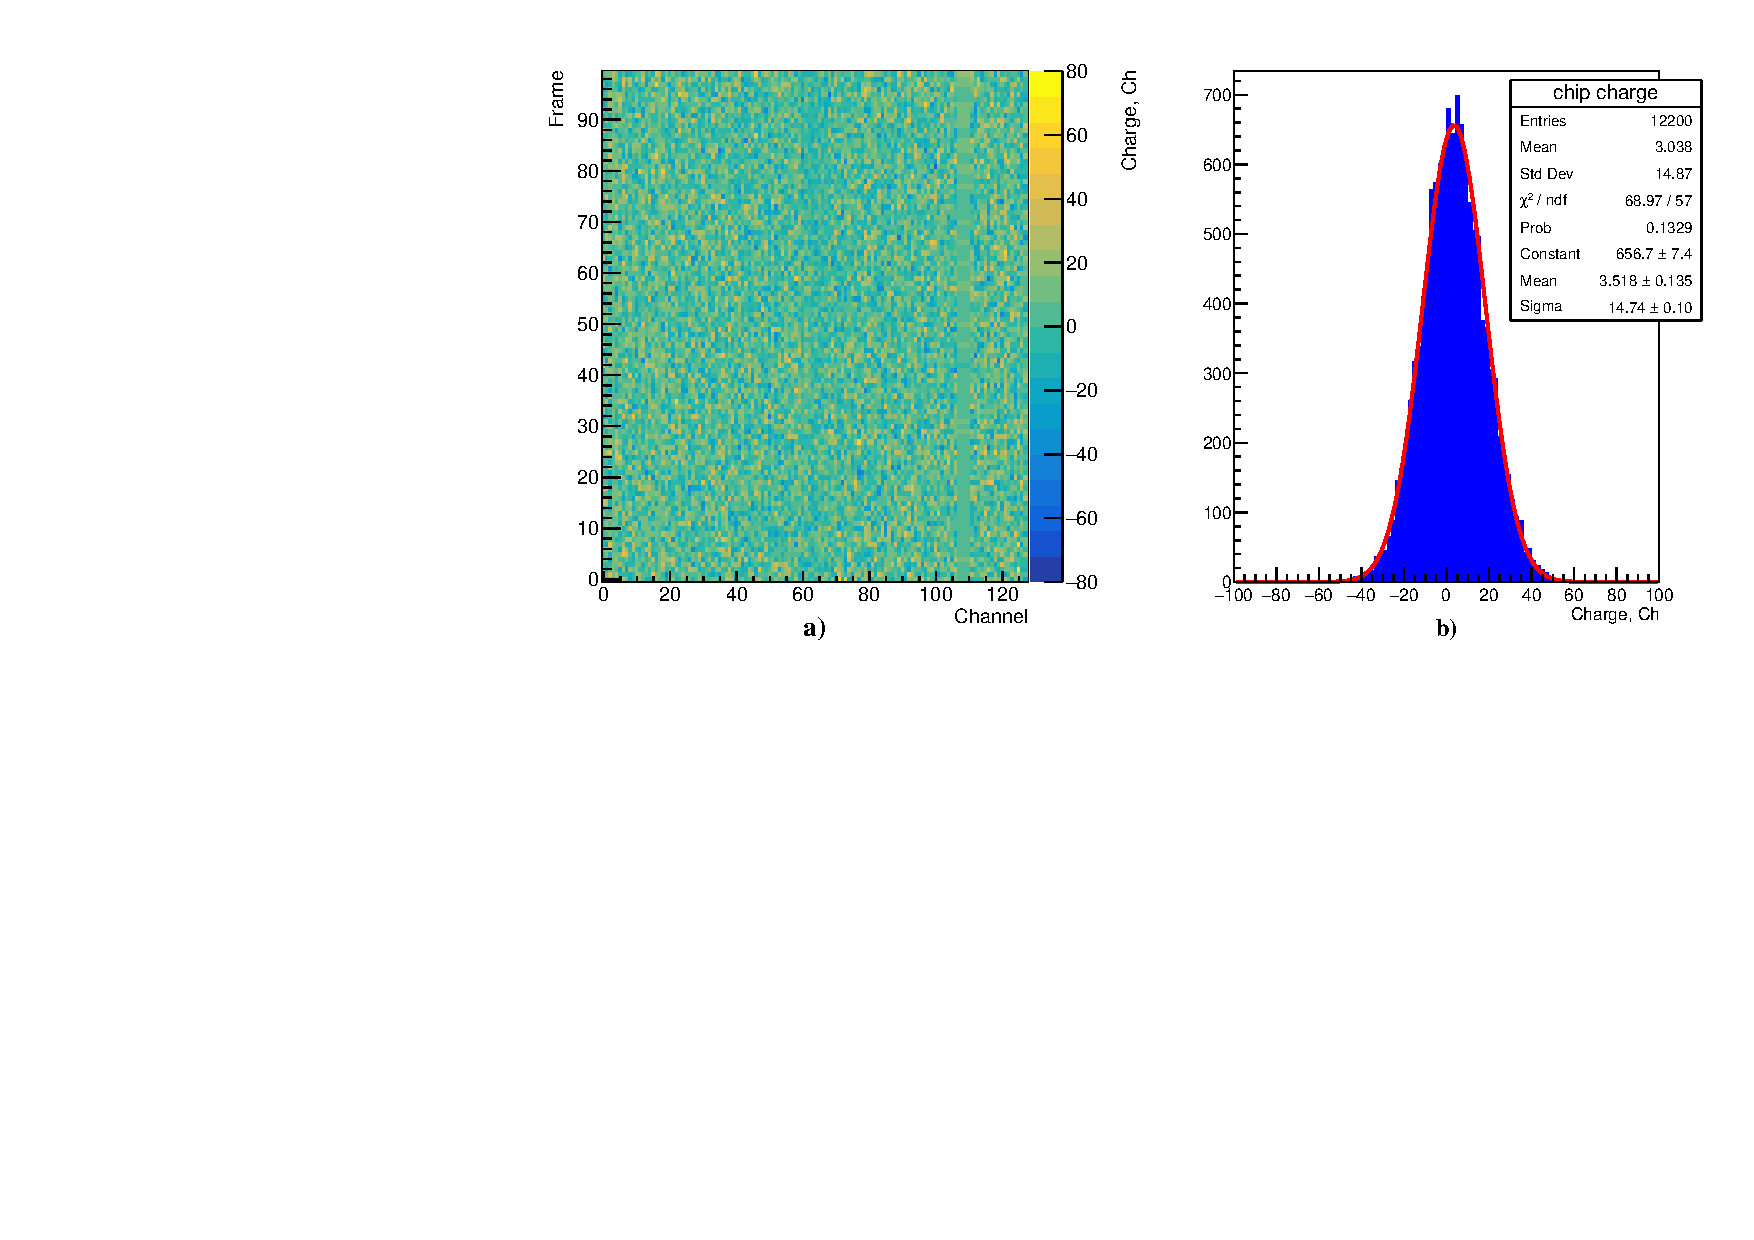
\includegraphics[width = 12cm]{img/noise_map.pdf}
		\caption{a): Вид шумового события после вычитания пьедестала b): Распределение заряда в шумовом событии}
		\label{noise_map}
	\end{center}
\end{figure}
Рис. \ref{noise_map} показывает вид одного шумового события и распределение заряда в кадрах и каналах. Важным значением, которое можно извлечь уже из одного шумового события является уровень шумов. Его можно определить как корень из дисперсии распределения на Рис. \ref{noise_map} b). Шумы в данном эксперименте составили $\approx15$ каналов АЦП. Если взять несколько шумовых событий, то можно уточнить данное значение. Более того, записывая данные через равные промежутки времени, можно зафиксировать наличие дрейфа уровня шумов и их среднего значения. Такое исследование тоже было проведено. Его результаты показали, что уровень шумов со временем меняется незначительно (Рис.\ref{fig:Noise_gr}.)

\begin{figure}[H]
\centering
\begin{subfigure}{.5\textwidth}
	\centering
	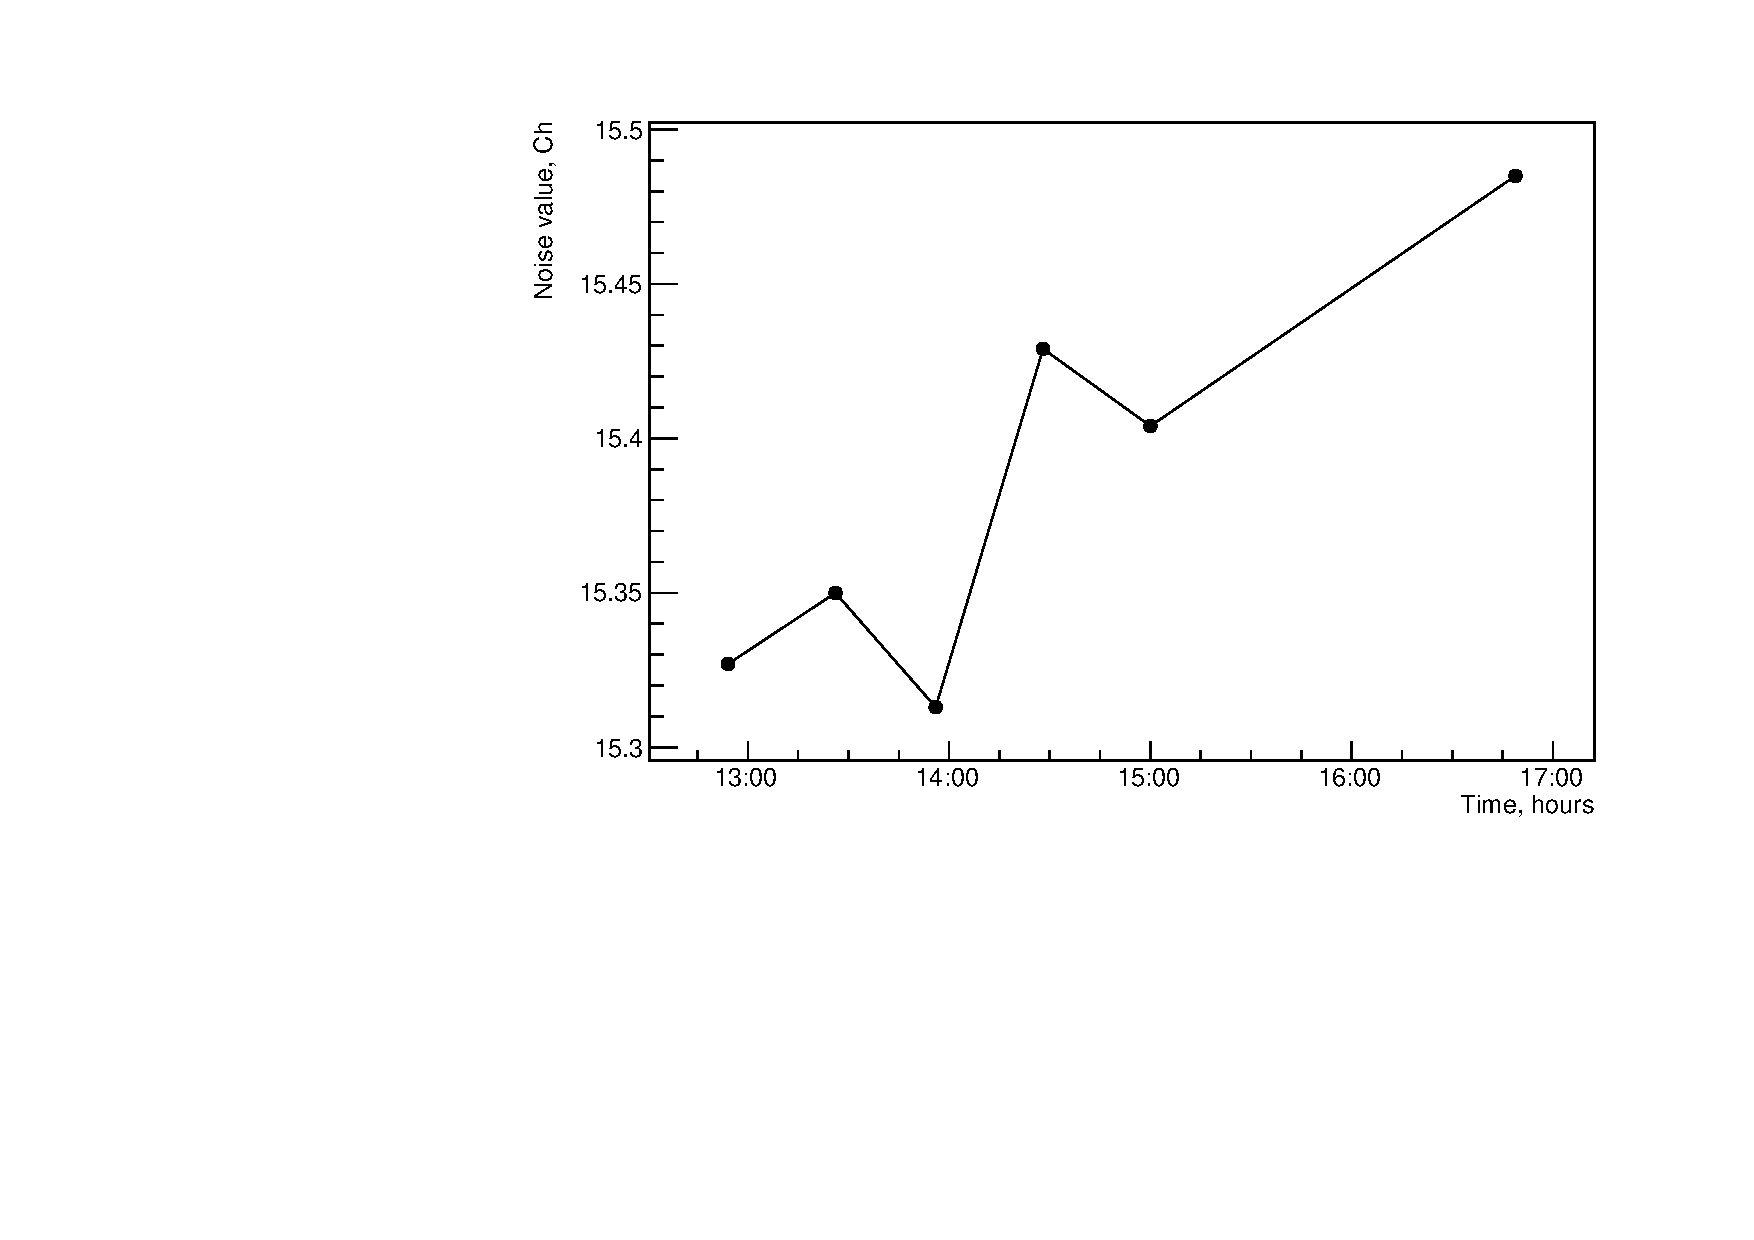
\includegraphics[width=1\linewidth]{img/Noise_time_drift.pdf}
	\caption{Уровень шумов}
\end{subfigure}%
\begin{subfigure}{.5\textwidth}
	\centering
	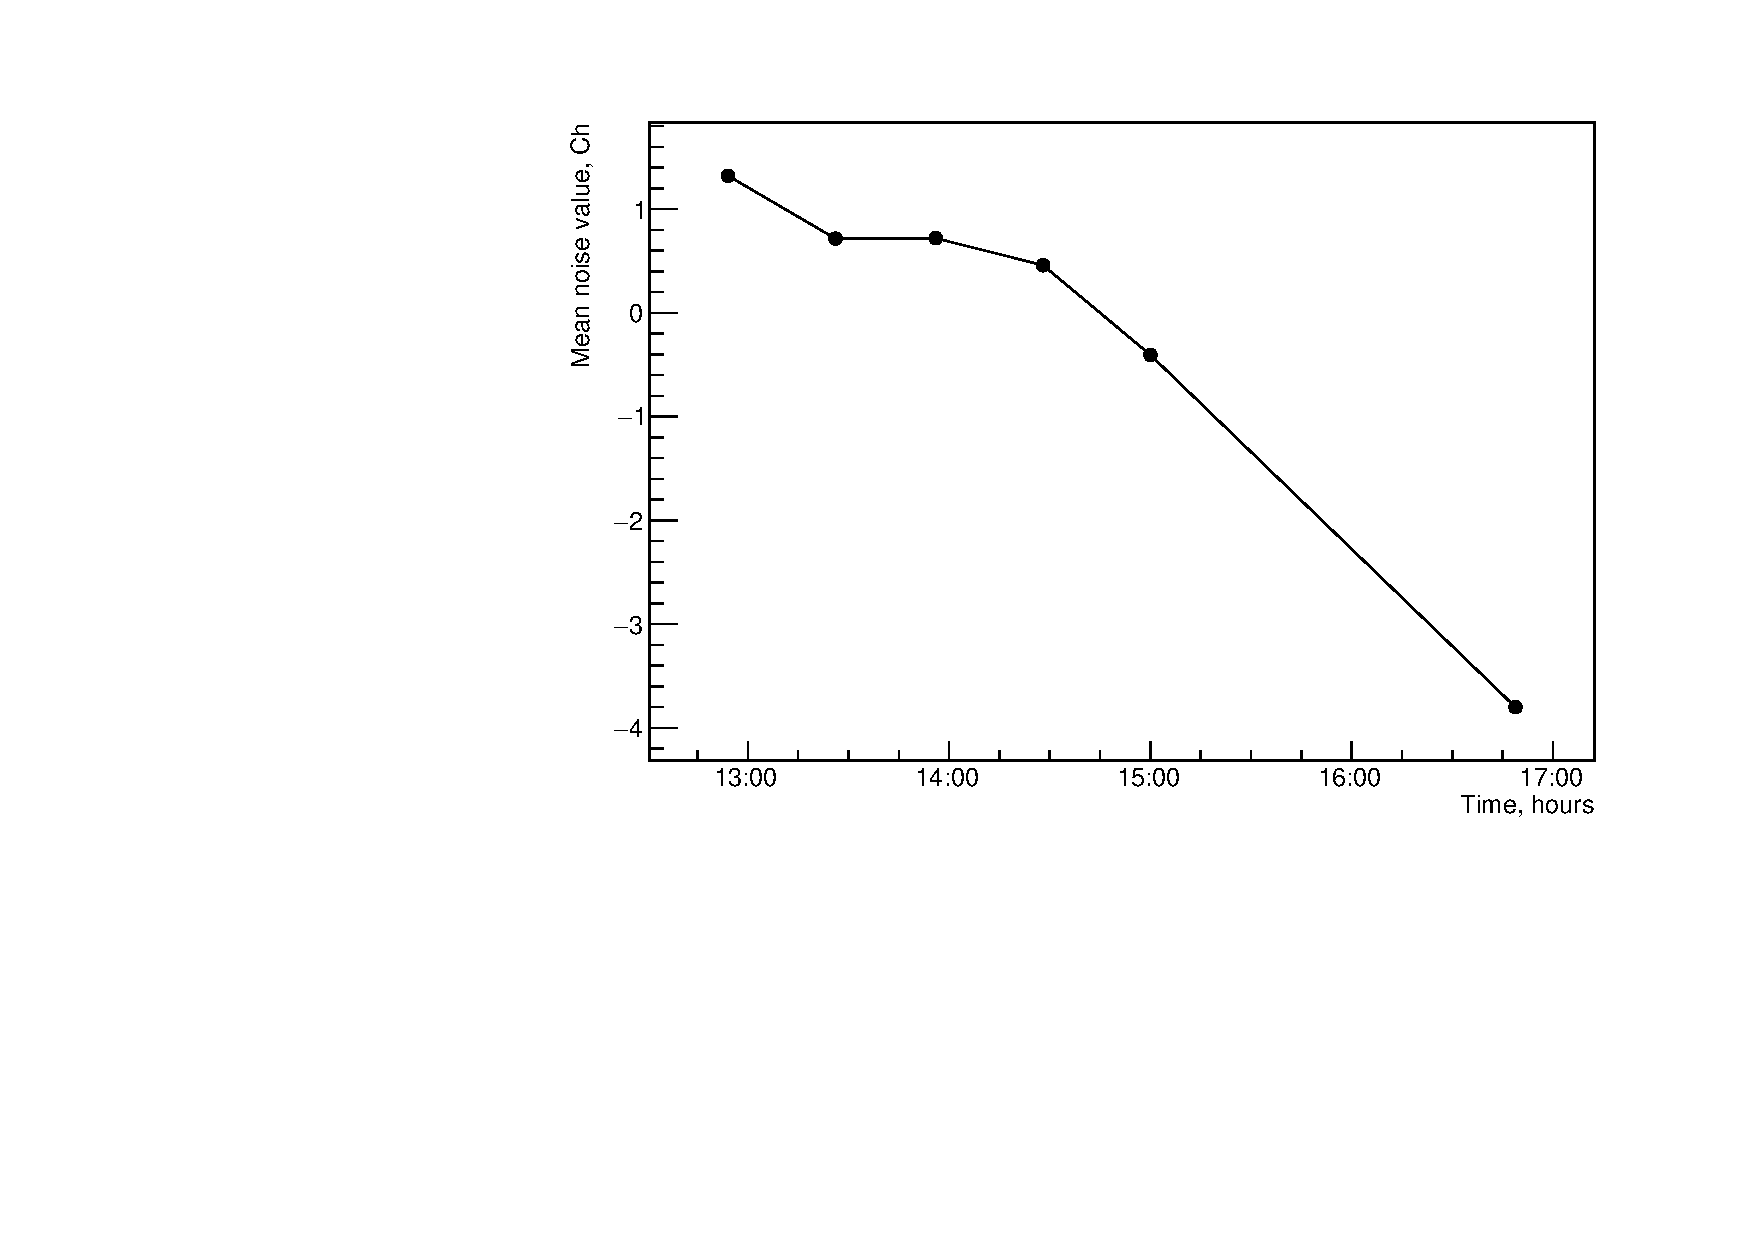
\includegraphics[width=1\linewidth]{img/Mean_time_drift.pdf}
	\caption{Среднее значение шума}
\end{subfigure}
\caption{Временной дрейф параметров шумовых событий: уровня шума и среднего значения шума. Каждая точка - среднее по $3\cdot10^7$ значений. В обоих случаях наблюдается линейный тренд.}
\label{fig:Noise_gr}
\end{figure}
Относительное изменение уровня шума за 4 часа составило 0.87 \%, а дрейф среднего значения -- 0.06 \%. Такими малыми изменениями можно пренебречь при дальнейшем анализе экспериментальных данных.  

\section{Обработка сигнальных событий}
Электронная лавина обычно регистрируется не одним каналом считывающей структуры, а несколькими. Это вызвано диффузией носителей в газовых промежутках детектора, что вызывает увеличение поперечных размеров области с носителями. Назовем такое распределение заряда от одной электронной лавины кластером. На мониторе события, который представлен на Рис. \ref{event_map}, можно видеть группы вертикальных желтых полос. Это и есть кластеры. Заряд в них экспоненциально убывает со временем. Для анализа же требуется только значение с первого кадра, где наблюдается превышение уровня заряда над фоном.   
\begin{figure}[H]
	\begin{center}
		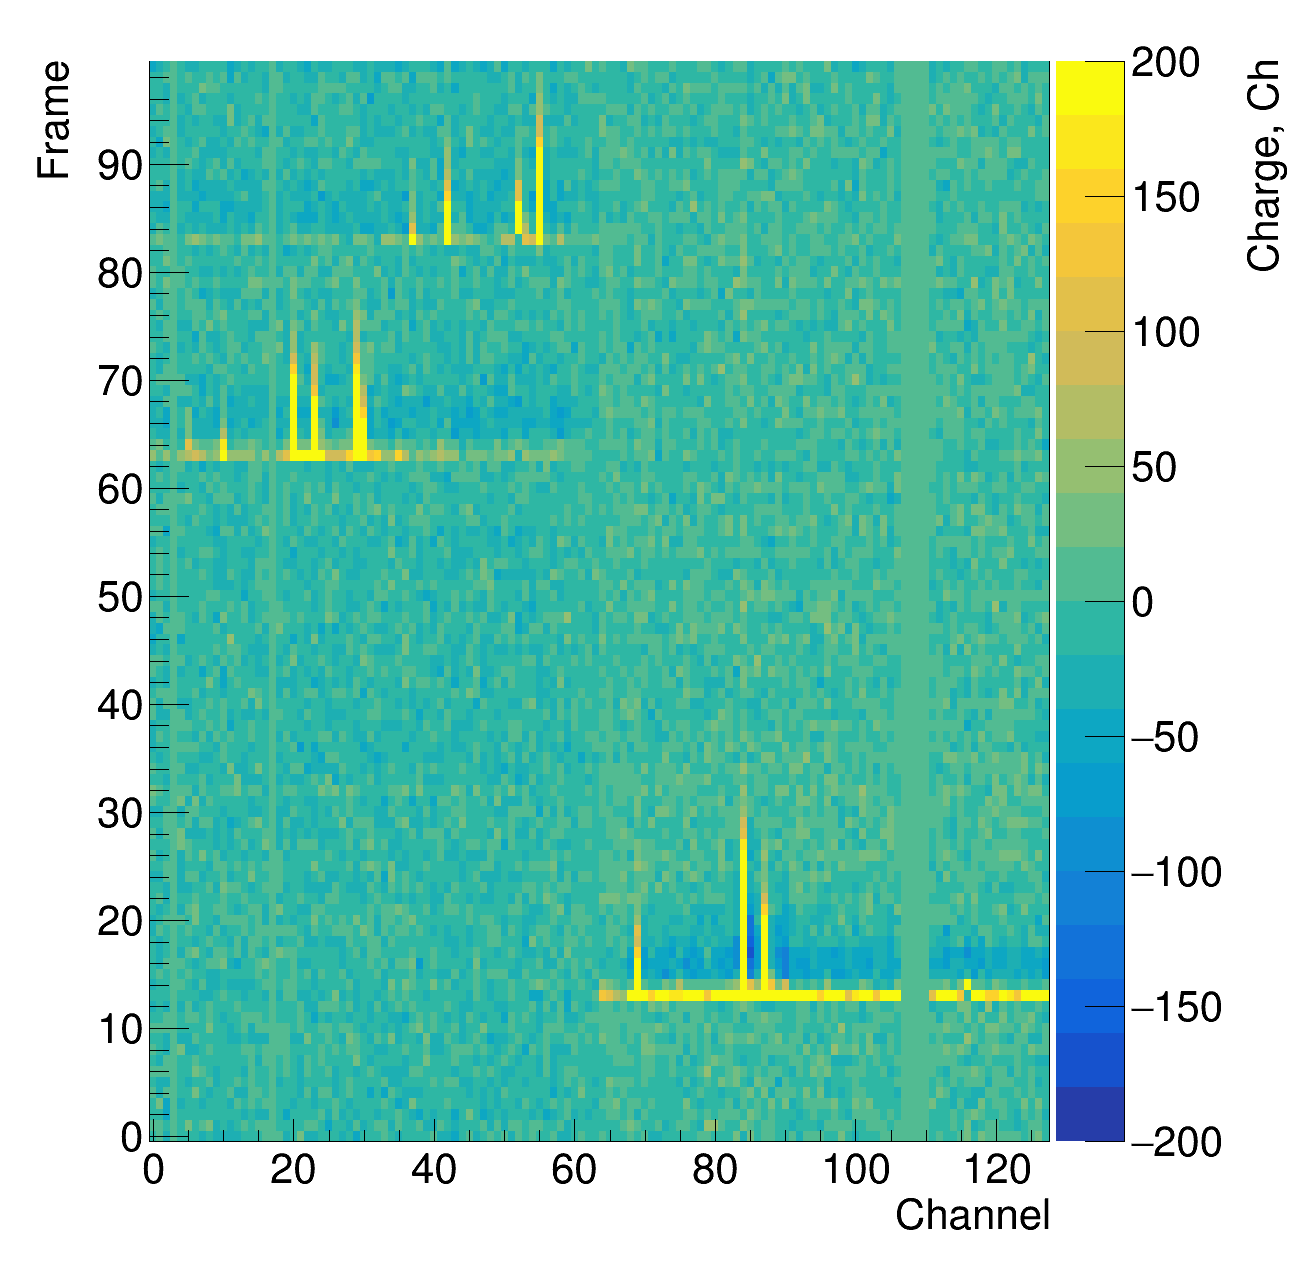
\includegraphics[width = 8cm, height = 7cm]{img/Signal.png}
		\caption{Вид сигнального события. По вертикальной оси отложены кадры, по горизонтальной - канале. Цвет показывает значение заряда в конкретном канале и кадре. В данном событии зафиксировано три кластера (два в первом чипе и один во втором)}
		\label{event_map}
	\end{center}
\end{figure}
 Заряд кластера является ключевой характеристикой при определении коэффициента усиления детектора. Поэтому необходим алгоритм, который ассоциирует группу каналов с кластером и вычисляет его заряд. С этой целью для детектора <<Лазерного поляриметра>> на языке Python написана библиотека, осуществляющая обработку первичных данных с детектора. В ней реализованы следующие алгоритмы:
 \begin{itemize}
 	\item предобработка данных события:
 	\begin{itemize}[label=$\circ$]
 		\item чтение файлов <<сырых данных>>
 		\item вычитание пьедесталов
 		\item маскировка шумовых каналов
 	\end{itemize}
 	\item фильтрация сигнальных событий
 	\item привязка номера канала АЦП к координатам считывающей площадки на плате
 	\item нахождение кластера и определение его заряда
 \end{itemize}
Особенности предобработки данных обсуждались выше (см. п. \ref{sec:DAQ_raw_data}). Рассмотрим работу остальных алгоритмов.
\par Чтобы привязать канал АЦП к координатам считывающей площадки, необходимо знать карту каналов. Она была получена путём прямого измерения и сверена со схемой считывающей платы. Необходимость измерения в первую очередь была продиктована высокой плотностью расположения электродов на плате, а так же необходимостью проверки работоспособности её электрических соединений. 
\begin{figure}[H]
	\centering
	\begin{subfigure}{.5\textwidth}
		\centering
		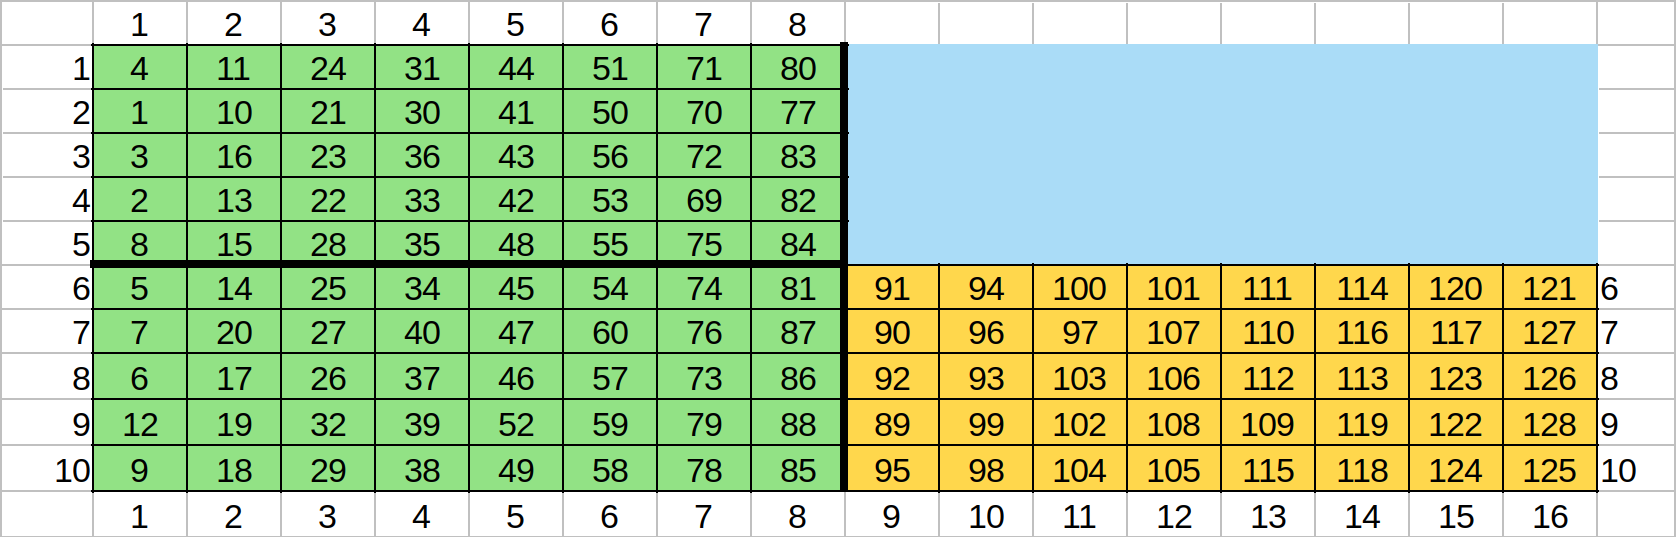
\includegraphics[height = 2.5cm]{img/Side_pixmap.png}
		\caption{Периферийная часть}
	\end{subfigure}%
	\begin{subfigure}{.5\textwidth}
		\centering
		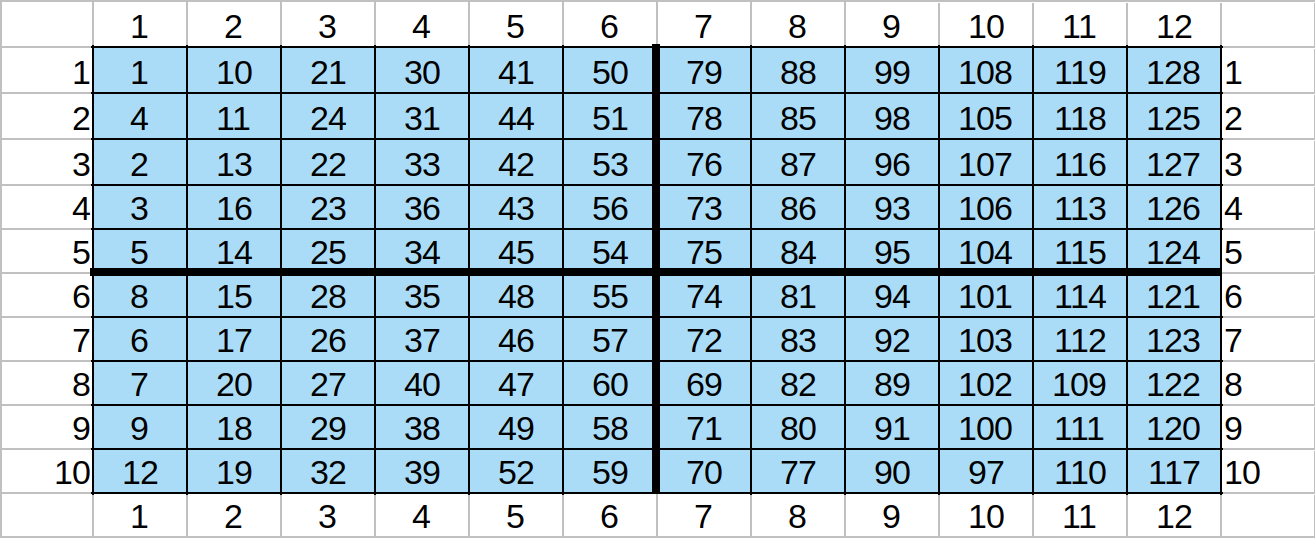
\includegraphics[height=2.5cm]{img/Center_pixmap.png}
		\caption{Центральная часть}
	\end{subfigure}
	\caption{Карты расположения считывающих площадок и номера каналов, которые им соответствуют. Представлено два случая расположения: для платы из периферийной и центральной областей. В цветных клетках указан номер канала АЦП, соответствующий данной считывающей площадке. Цифры вокруг цветной области - координаты считывающих площадок.}
	\label{fig:pixmap}
\end{figure}
Возьмем для примера центральную область. Считанное из файла событие преобразуется во временный двумерный массив ($128\times100$), а затем в соответствии с картой каналов данные из него перегружаются в трехмерный массив ($12\times10\times100$), первые две координаты массива соответствуют координатам считывающей структуры. Восемь каналов: $60\div67$ не используются, и входы АЦП, соответствующие им, не подключены к считывающей структуре. Дальнейшая работа проводится с этим трехмерным массивом.
\par В ходе работы было обнаружено, что при регистрации кластера с большим значением заряда нулевой уровень шумовых каналов смещается. Результат этого виден на Рис. \ref{event_map}, где средний уровень кадра находится в желтой области, что говорит о его смещении на 100-200 каналов. Т.к. при регистрации кластера этот систематический сдвиг будет смещать значение каждого канала, то суммарная ошибка определения заряда кластера возрастёт в $\sqrt{N_{Ch}}$ раз, где $N_{Ch}$ -- количество сработавших каналов. Поэтому необходимо каким-то образом произвести поправку на систематический сдвиг нулевого уровня заряда для каждого кадра.
\begin{figure}[H]
	\centering
	\begin{subfigure}{.33\textwidth}
		\centering
		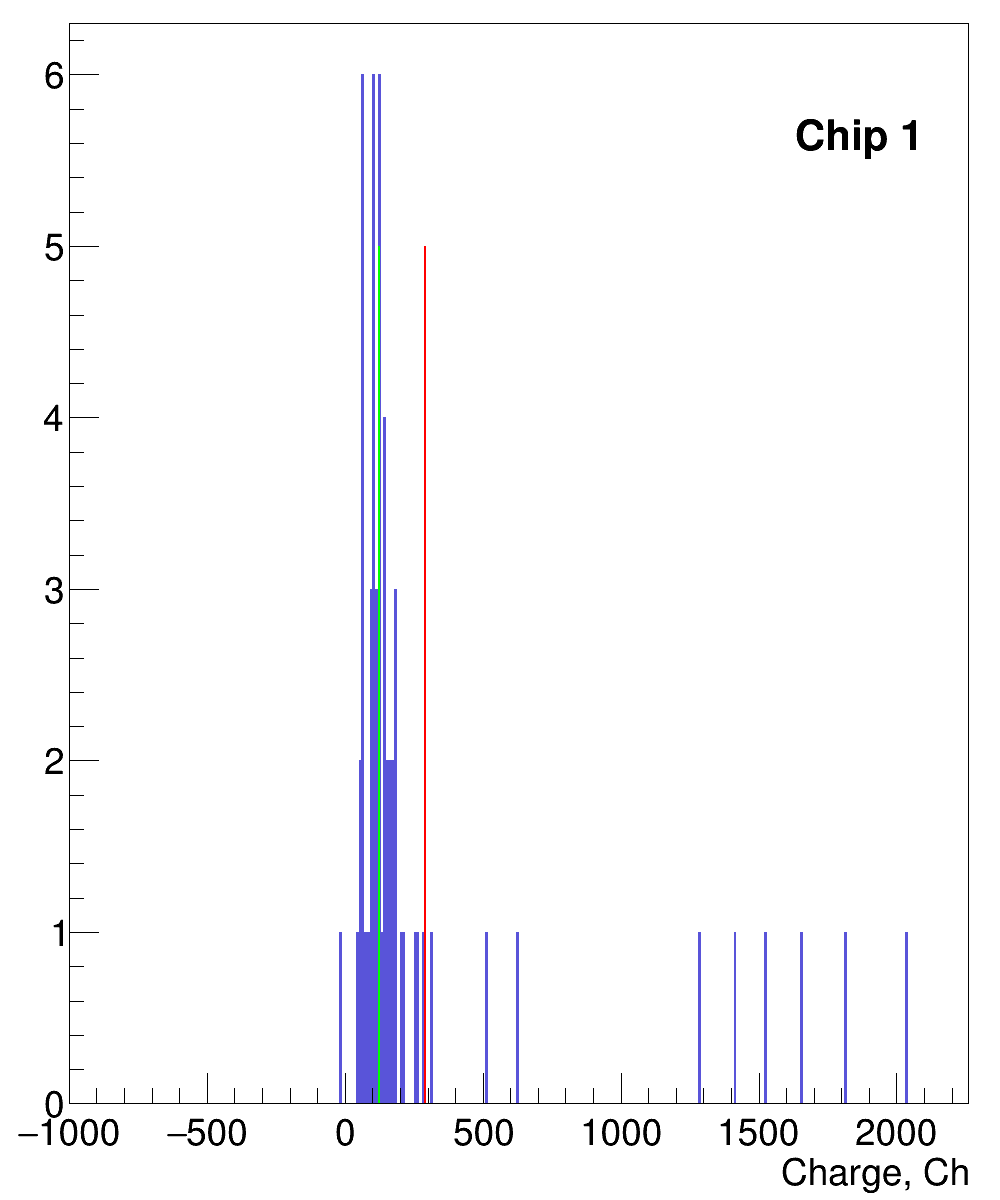
\includegraphics[height = 6.5 cm, width= 5.5cm]{img/Median_unzoomed.png}
		\caption{Распределение заряда\\в кадре}
		\label{fig:median_signal}
	\end{subfigure}%
	\begin{subfigure}{.33\textwidth}
		\centering
		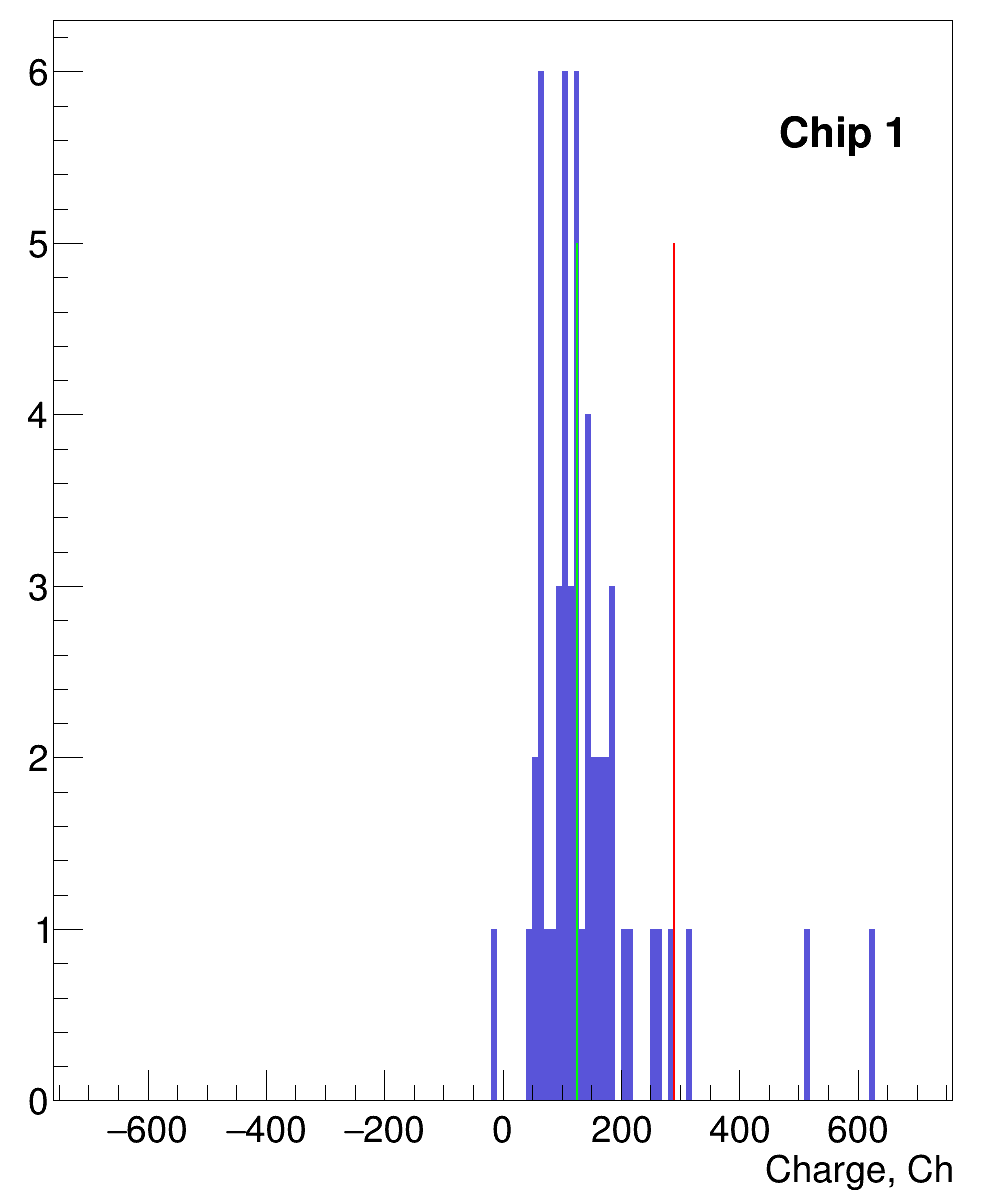
\includegraphics[height = 6.5 cm, width= 5.8cm]{img/Median_1.png}
		\caption{Шумовые каналы \\ (без~фильтра)}
		\label{fig:median_noize}
	\end{subfigure}
	\begin{subfigure}{.33\textwidth}
		\centering
		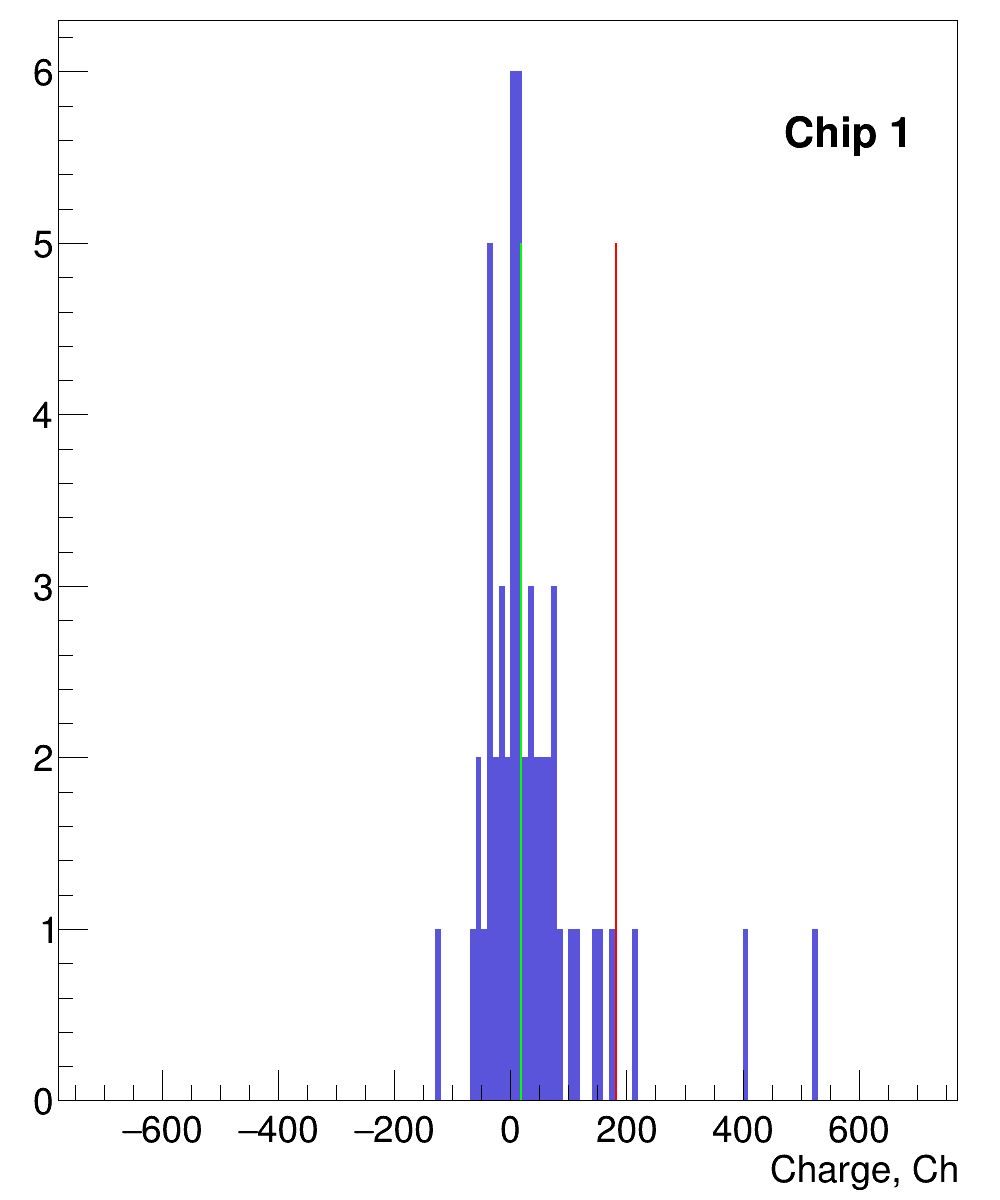
\includegraphics[height = 6.5 cm, width= 5.8cm]{img/Median_0.png}
		\caption{Шумовые каналы\\(с~фильтром)}
		\label{fig:medianF_noize_biased}
	\end{subfigure}%
	\caption{Распределение заряда в сигнальном кадре. Красная вертикальная линия показывает среднее значение по распределению. Зеленая -- медиану распределения. Медиана дает более точную оценку среднего по шумам, что позволяет сделать поправку и сместить средний уровень кадра к нулю.}
	\label{fig:medianF}
\end{figure}
Если построить распределение по заряду в каналах одного кадра, то можно заметить, значения заряда шумовых каналов  сгруппированы вблизи нуля, а заряд от сигнальных каналов находится далеко справа от нуля (Рис. \ref{fig:median_signal}.) Более того, на Рис. \ref{fig:median_noize} виден сдвиг среднего значения шумов относительно нуля. Можно заметить, что использование обычного порогового фильтра в данном случае малоэффективно по двум причинам:
\begin{enumerate}
	\item Систематический сдвиг нулевого значения канала может стать причиной ошибочного распознования шумовых каналов, как сигнальных
	\item При малом заряде кластера сигнальные каналы могут быть приняты за шумовые
\end{enumerate}
Так же непонятно, как определять пороговое значение для разделения сигнала и шума? Для решения этой задачи была реализована идея медианного алгоритма, графическое представление которой можно видеть на Рис.\ref{fig:medianF}. Суть алгоритма заключается в вычислении медианы распределения по заряду для отдельного кадра. Причем при небольшом количестве сработавших каналов медиана достаточно точно описывает среднее значение заряда по шумовым каналам, которое, после вычитывания пьедесталов, должно равняться нулю. Если сдвинуть значение заряда в каждом канале на вычисленную медиану, то это позволяет подавить систематический сдвиг нулевого уровня в кадре. 
